\documentclass{beamer}
\usetheme{Warsaw}
\definecolor{mybg}{RGB}{240,240,255}
\setbeamercolor{background canvas}{bg=mybg}
\usepackage[polish]{babel}
\usepackage[utf8]{inputenc}
\usepackage[T1]{fontenc}

\title{Samoloty}
\author{Jan Jus}
\begin{document}

\begin{frame}
\titlepage
\end{frame}

\begin{frame}{Airbus a320neo}
\begin{figure}
    \centering
    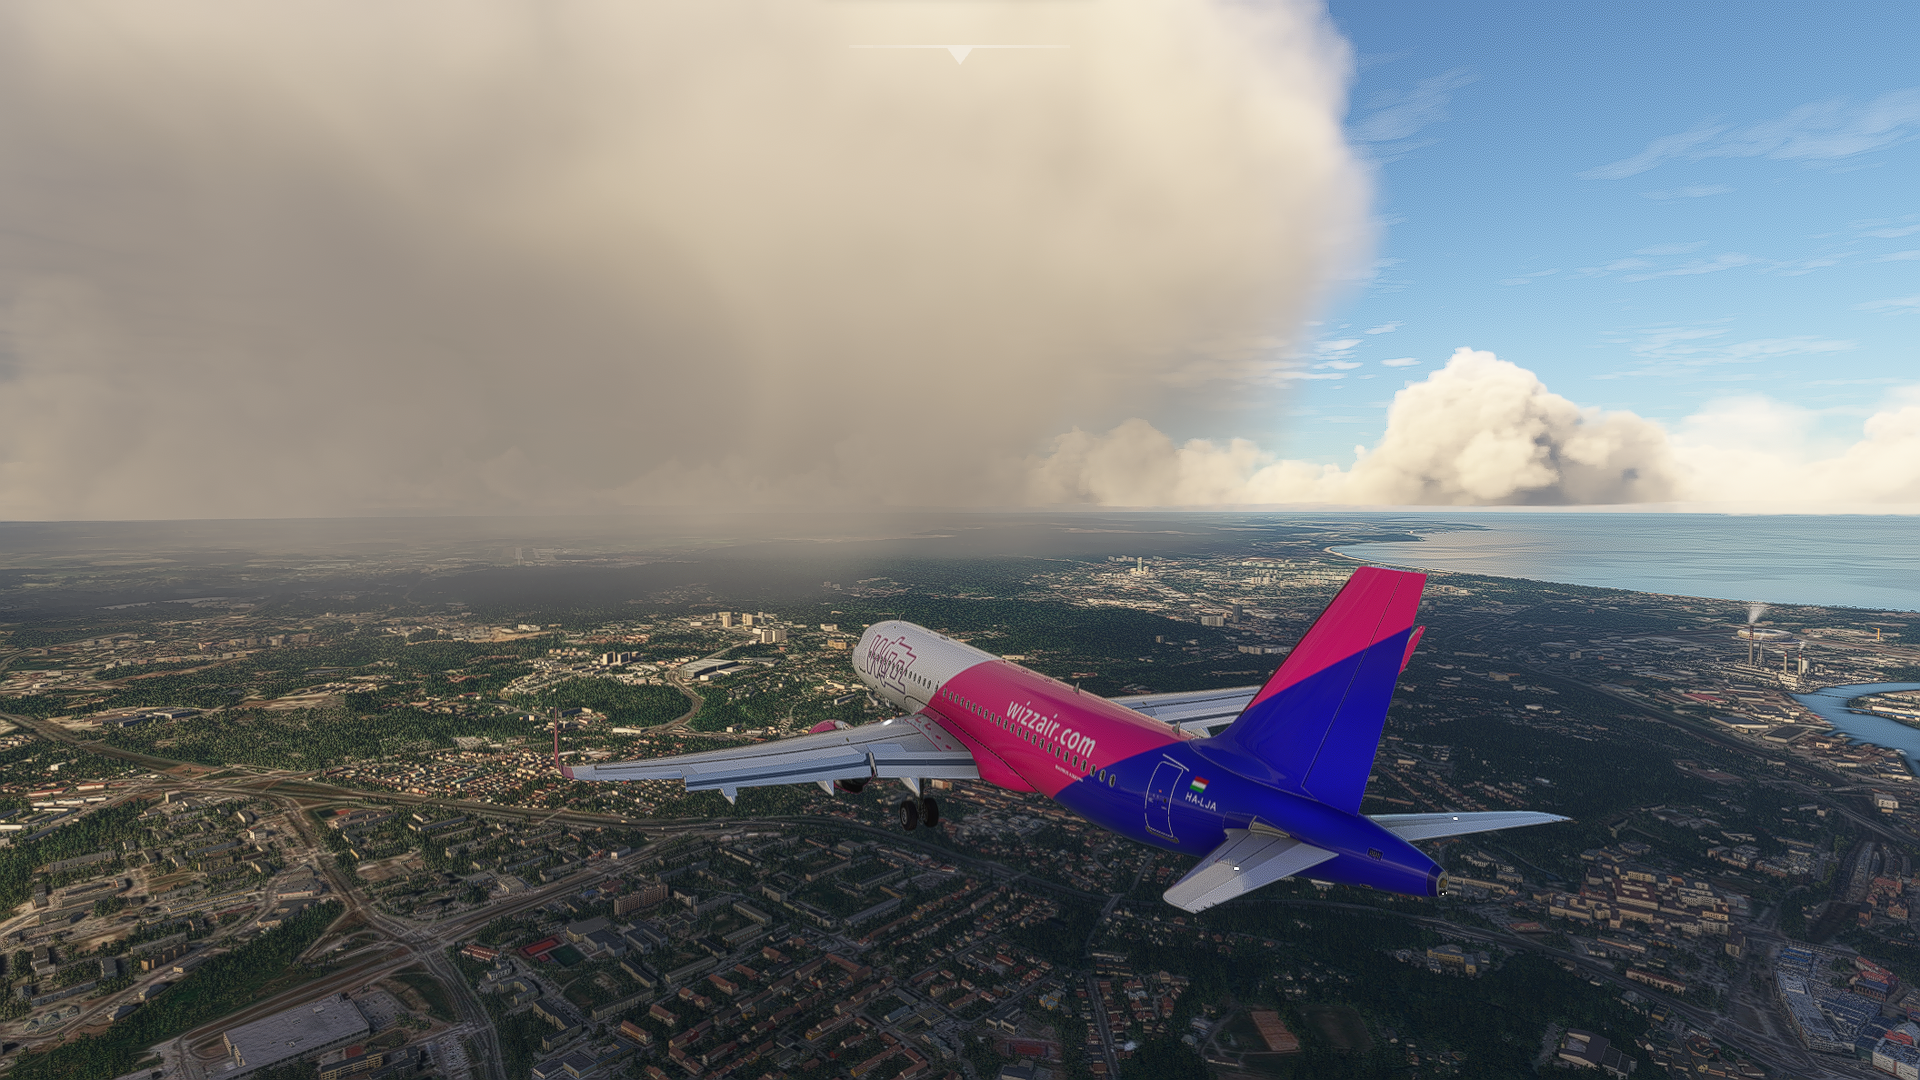
\includegraphics[width=0.5\textwidth]{landing.png}
    \caption{Airbus a320neo}
    \end{figure}
  \label{pic:pic1}
\end{frame}


\begin{frame}{Airbus a320neo}
\begin{figure}
    \centering
    \includegraphics[width=0.5\textwidth]{left.png}
    \caption{Airbus a320neo}
    \end{figure}
  \label{pic:pic2}
\end{frame}


\begin{frame}{Airbus a320neo}
\begin{figure}
    \centering
    \includegraphics[width=0.5\textwidth]{right.png}
    \caption{Airbus a320neo}
    \end{figure}
  \label{pic:pic3}
\end{frame}


\begin{frame}{Airbus a320neo}
\begin{figure}
    \centering
    \includegraphics[width=0.5\textwidth]{top.png}
    \caption{Airbus a320neo}
    \end{figure}
  \label{pic:pic4}
\end{frame}


\begin{frame}{Airbus a380-861}
\begin{figure}
    \centering
    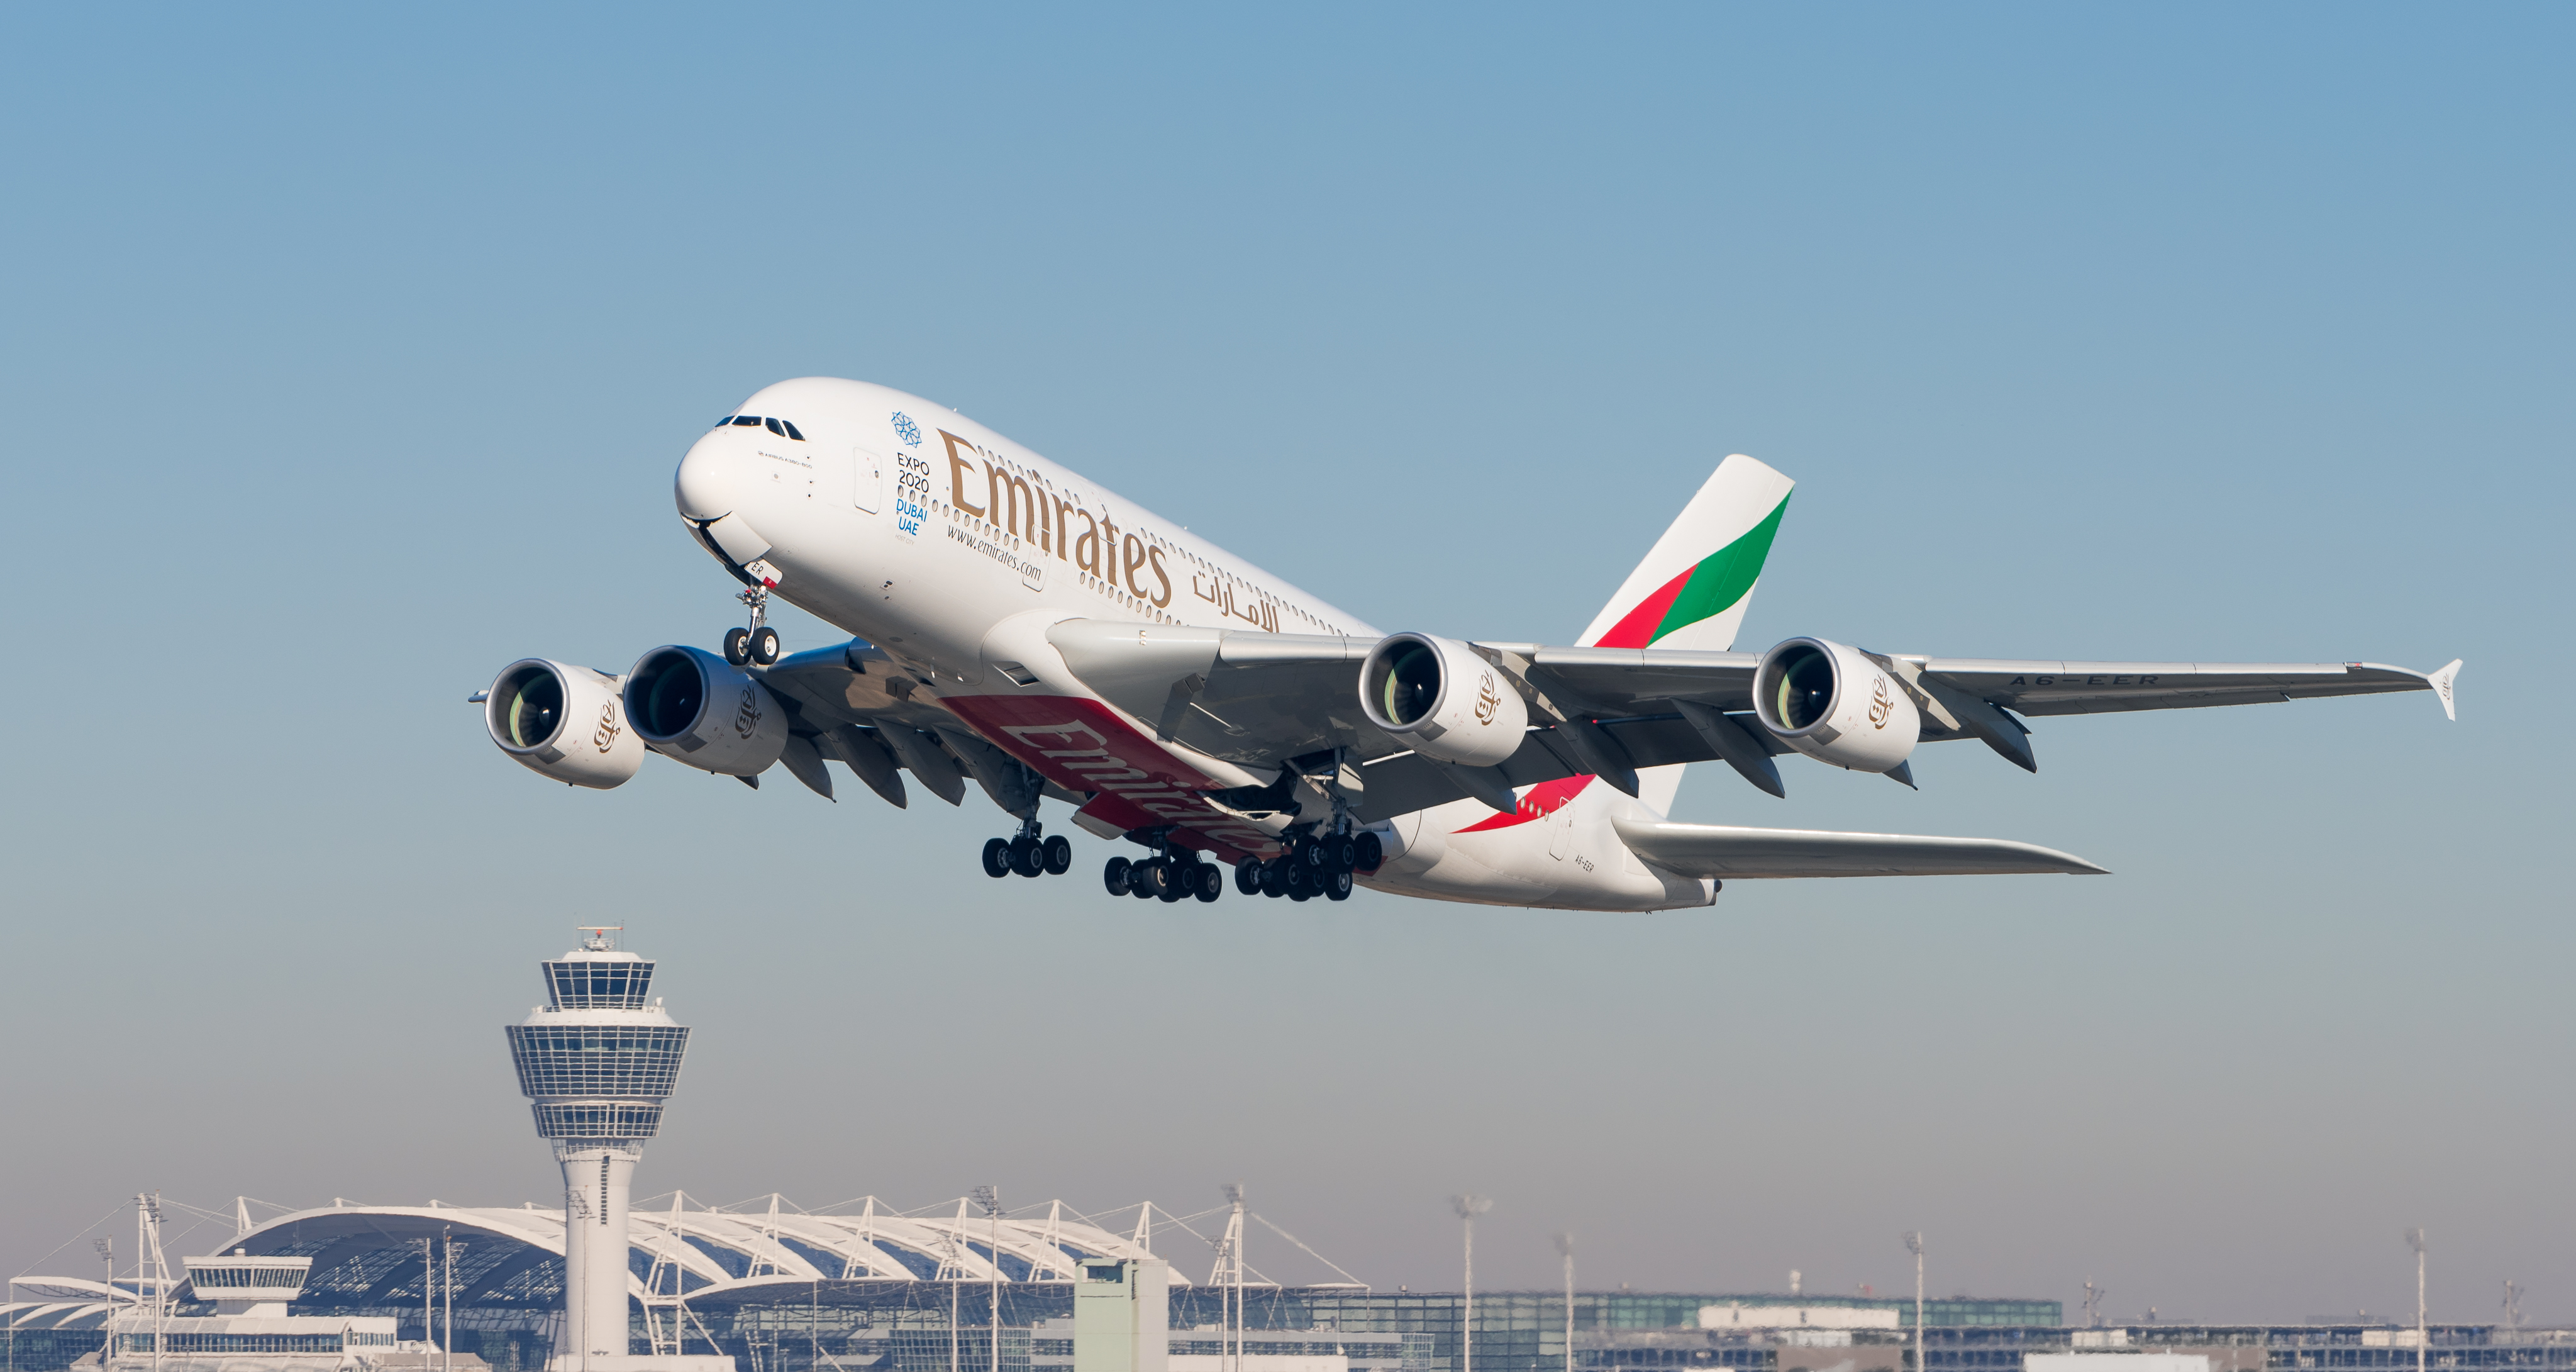
\includegraphics[width=0.5\textwidth]{a380.jpg}
    \caption{Airbus a380-861}
    \end{figure}
  \label{pic:pic5}
\end{frame}


\begin{frame}{Bombardier Dash 8 Q400}
\begin{figure}
    \centering
    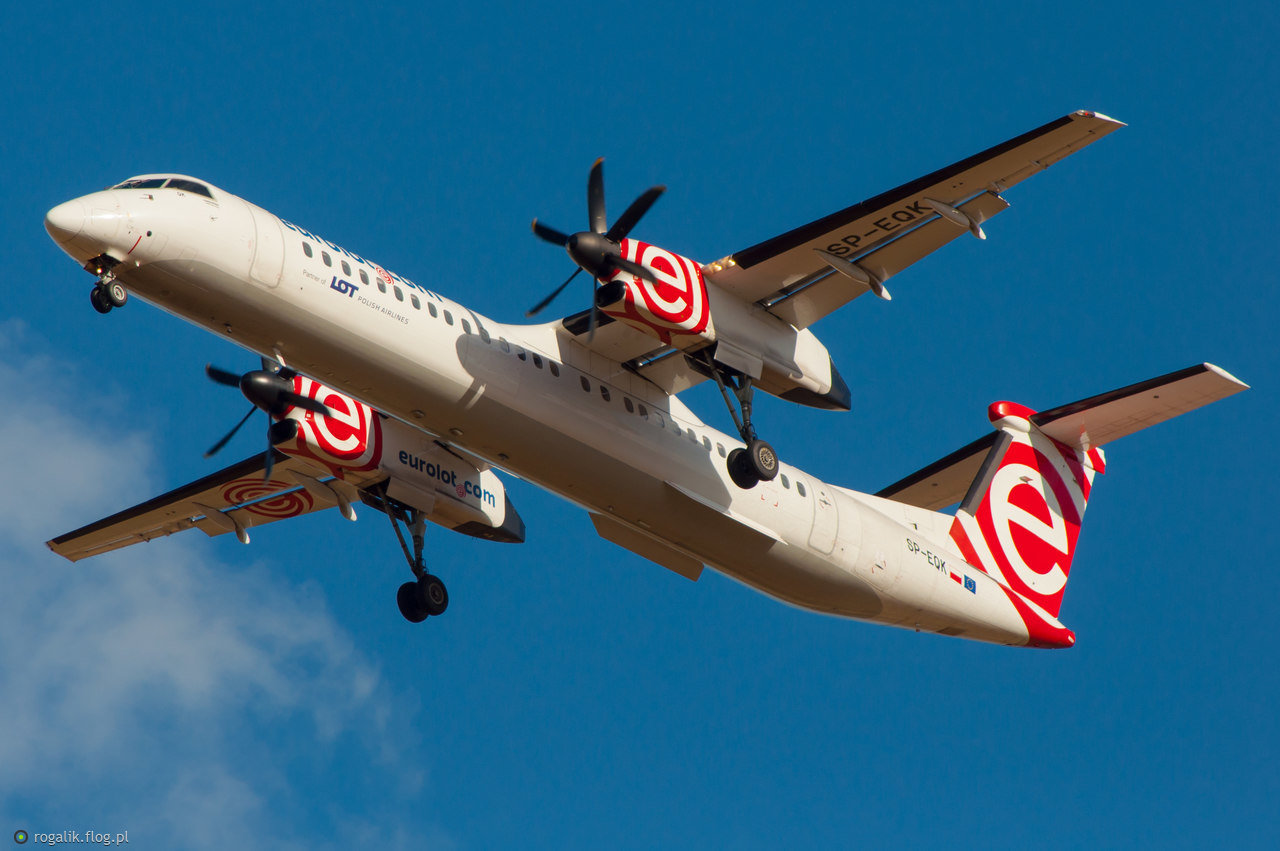
\includegraphics[width=0.5\textwidth]{dash8.jpg}
    \caption{Bombardier Dash 8 Q400}
    \end{figure}
  \label{pic:pic6}
\end{frame}


\begin{frame}{Boeing 737-800}
\begin{figure}
    \centering
    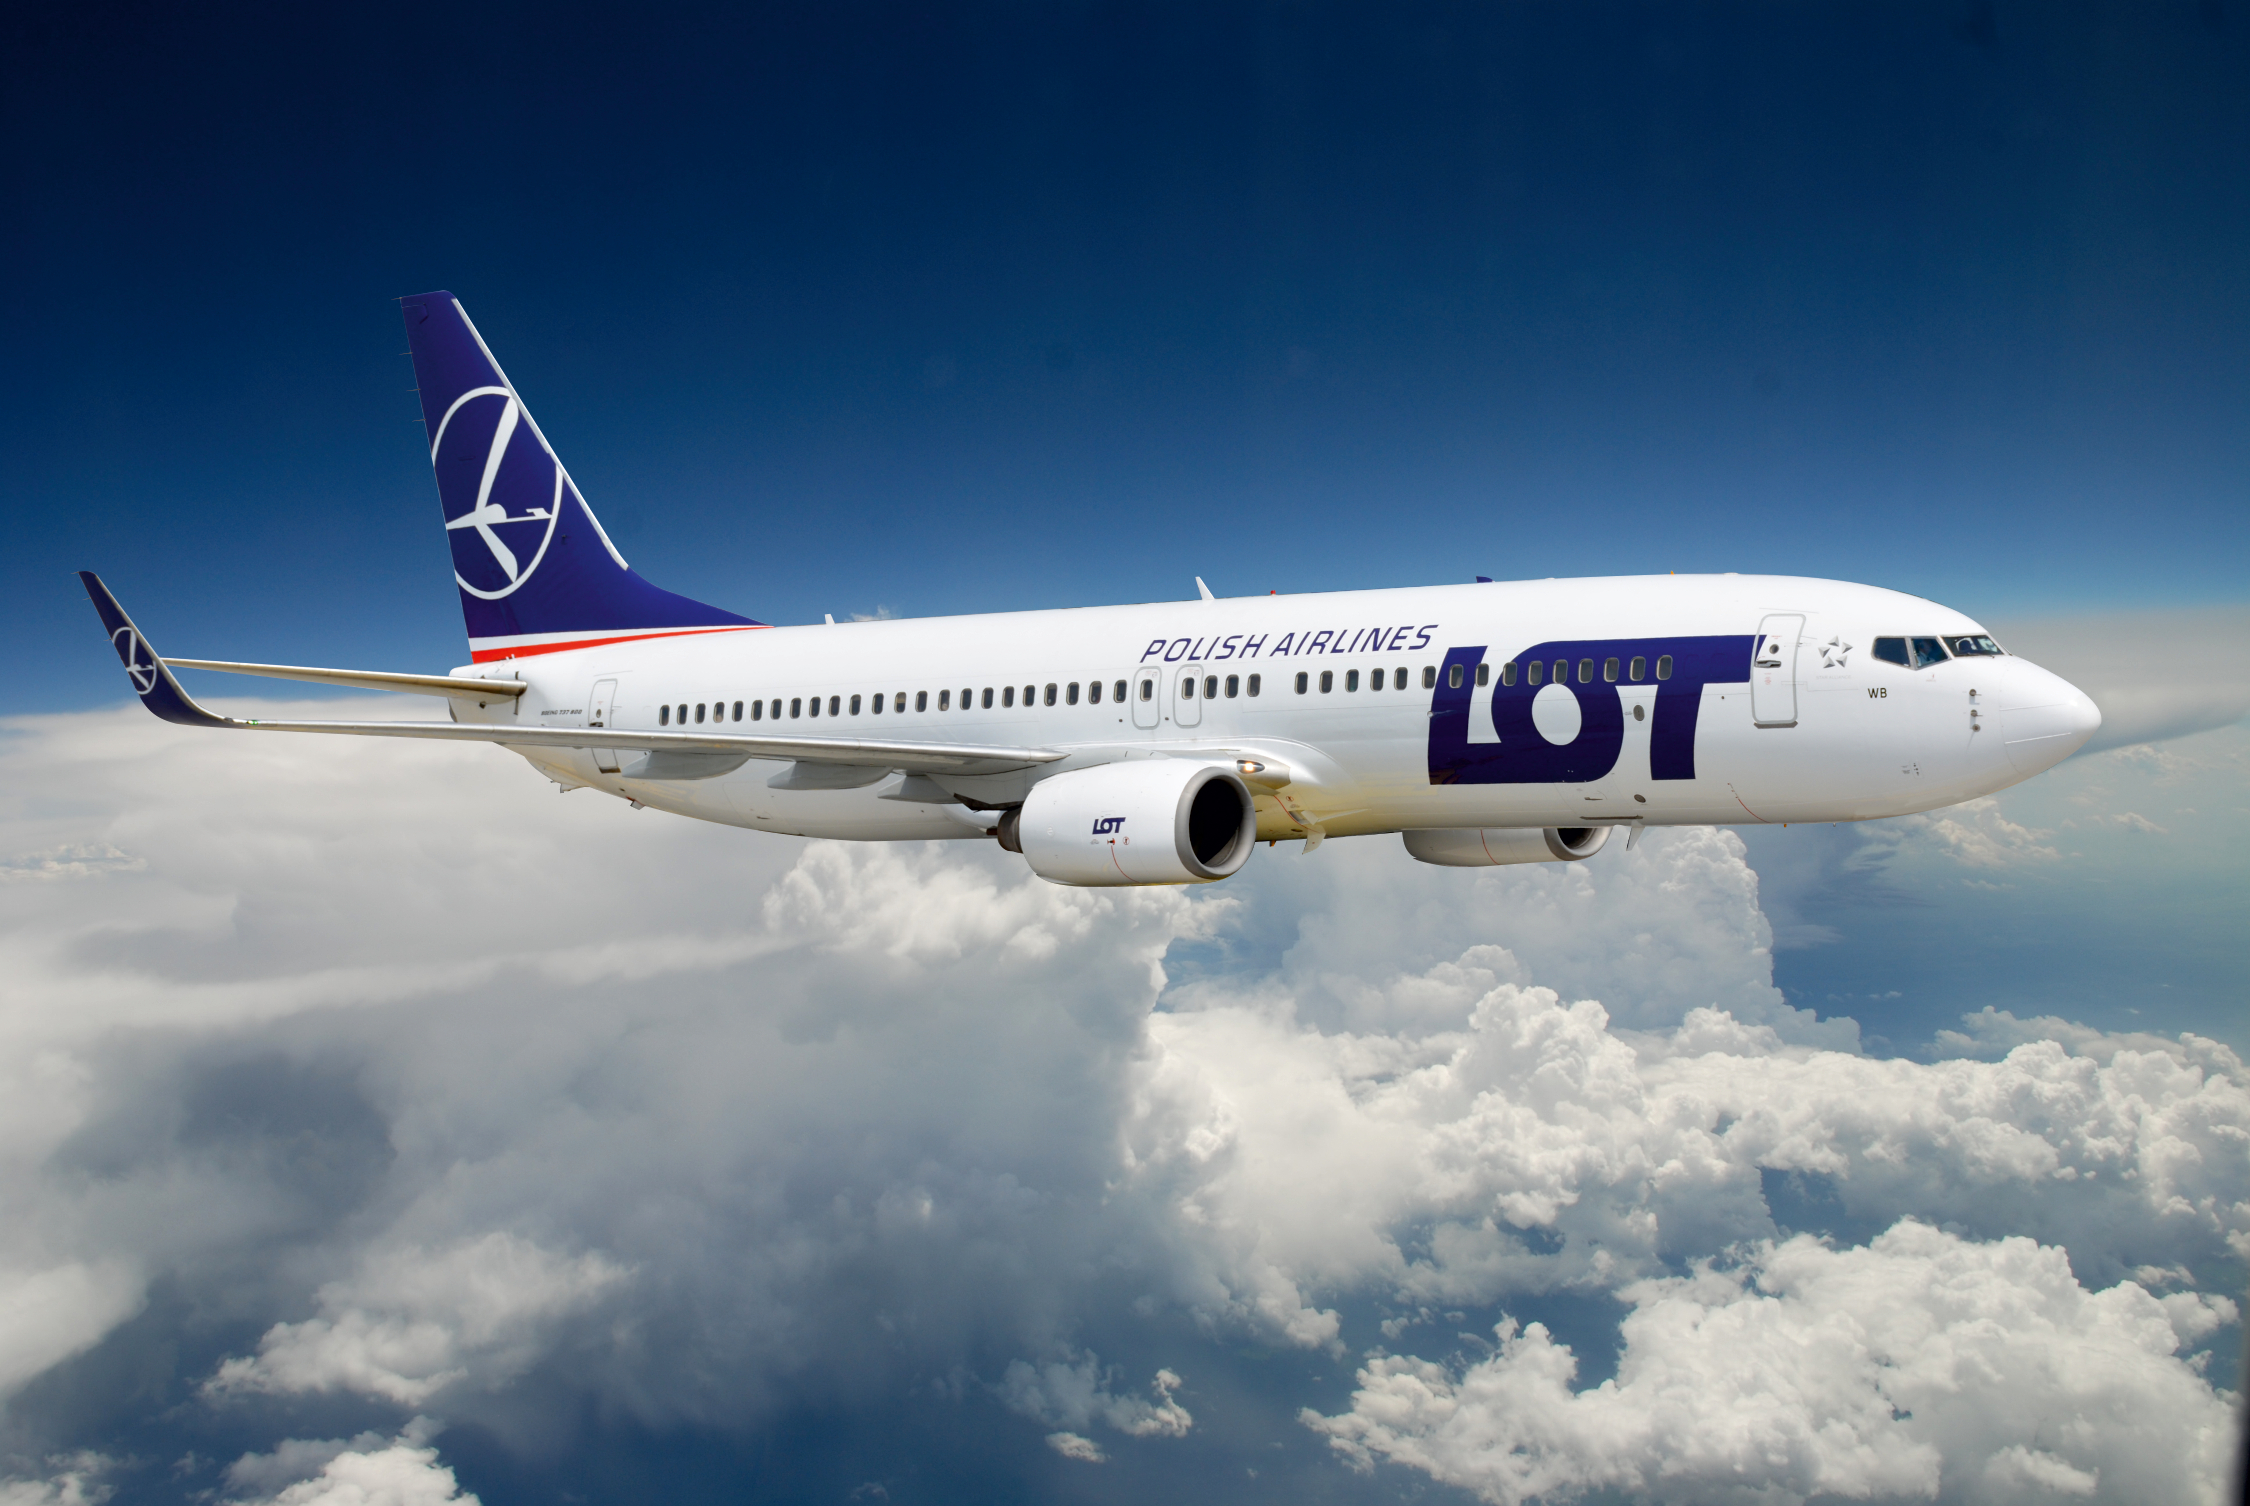
\includegraphics[width=0.5\textwidth]{b7378.jpg}
    \caption{Boeing 737-800}
    \end{figure}
  \label{pic:pic7}
\end{frame}


\begin{frame}{Porównanie samolotów}
\centering
\begin{tabular}{|c|c|}
\hline
Samolot & Rok produkcji \\
\hline
Airbus A380-861 & 2007 \\
\hline
Boeing 737 Max8 & 2017 \\
\hline
Boeing 747-400 & 1988 \\
\hline
Boeing 787-900 & 2011 \\
\hline
Boeing 737-800 & 1998 \\
\hline
Airbus A340-300 & 1991 \\
\hline
Bombardier Dash 8 Q400 & 2000 \\
\hline
\end{tabular}
  \label{tab:tab1}
\end{frame}

\begin{frame}{Dlaczego samoloty?}
\begin{enumerate}[a)]
\item Ponieważ są najbezpieczniejsze
\pause
\item Ponieważ są najszybsze
\pause
\item Ponieważ są duże
\pause
\item Ponieważ są najdroższe :D
\end{enumerate}
  \label{en:en1}
\end{frame}


\begin{frame}
\frametitle{Ranking najlepszych linii lotniczych}
\begin{enumerate}[1)]
\item Qatar Airways
\pause
\item Singapore Airlines
\pause
\item ANA All Nippon Airways
\pause
\item Cathay Pacific
\pause
\item Emirates
\end{enumerate}
  \label{en:en2}
\end{frame}


\begin{frame}
\frametitle{Najbardziej popularne samoloty}
\begin{enumerate}[1)]
\item Boeing 737
\pause
\item Airbus A320
\pause
\item Airbus A321
\pause
\item Boeing 747
\pause
\item Boeing 767
\end{enumerate}
  \label{en:en3}
\end{frame}

\begin{frame}
\frametitle{Bibliografia i odwołania do tabeli/rysunków}
\begin{itemize}
\item Odwołania do zdjęć i tabel: \ref{pic:pic1}, \ref{pic:pic2}, \ref{pic:pic3}, \ref{pic:pic4}, \ref{pic:pic5}, \ref{pic:pic6}, \ref{pic:pic7}, \ref{tab:tab1}, \ref{en:en1}, \ref{en:en2}, \ref{en:en3}
\end{itemize}
\begin{itemize}
\item Źródła:
\end{itemize}
\href{https://www.worldairlineawards.com/award/worlds-best-airline/}{\ref{en:en2} World's Best Airlines}
\href{https://www.aircraftcompare.com/news/the-most-popular-aircraft-types-in-the-world/}{\ref{en:en3} Most Popular Aircraft Types}
\end{frame}


\end{document}